\documentclass{article}
\usepackage{titlesec}
\usepackage{verbatim}
%provides multi-line comment syntax : \begin{comment} \end{comment}
\usepackage[xetex]{graphicx}

\begin{comment}
\titleformat{\section}[runin]
  {\normalfont\Large\bfseries}{\thesection}{1em}{}
\titleformat{\subsection}[runin]
  {\normalfont\large\bfseries}{\thesubsection}{1em}{}
\titleformat{\subsubsection}[runin]
  {\normalfont\large\bfseries}{\thesubsection}{1em}{}
\end{comment}



\title{NASA hw2}
\author{B04902045 孫凡耘}
\date{\today}

\begin{document}
\maketitle
    \section{Network Administration}
    \subsection{1}
    Modern Ethernet networks often use network switches to connect their links rather than hub right now. Since each link that connects to the switch has its own separate port, multiple access MAC protocol is no longer useful. For example, 10 Gibabit Ethernet removed this protocol. Instead, it uses network switches to achieve full duplex point-to-point links.
    \subsection{2}
    After aborting (that is, transmitting the jam signal), the adapter enters an exponential backoff phase. Specifically, when transmitting a given frame, after experiencing the nth collision in a row for this frame, the adapter chooses a value for K at random from \{0,1,2, . . . , 2m - 1\} where m = min(n,10). The adapter then waits K * 512 bits times.  \newline\newline
    n = 5, Probability: ${1 \over 32}$ \newline\newline
    Delay(K=4): ${4*512 bits\over 10 Mbps} = 2.048*10^{-4} $ s
    \newpage
    \subsection{3}
        Basically, I used the same command overall.\newline
        Workstation(server): iperf -s\newline
        PC(client): iperf -c \textless serverIP\textgreater \space\space -t 120 -i 10\newline
        120 seconds to transmit, pause 10 seconds between bandwidth report

        \subsubsection{csie wifi}
            \begin{figure}[!htb]
                \begin{flushleft}
                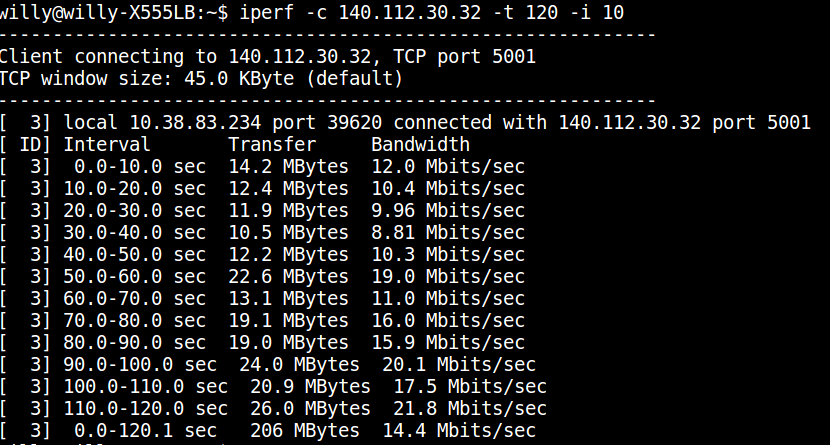
\includegraphics[scale=0.4]{csie_wifi.png}
                \end{flushleft}
            \end{figure}
            \begin{figure}[!htb]
                \begin{flushleft}
                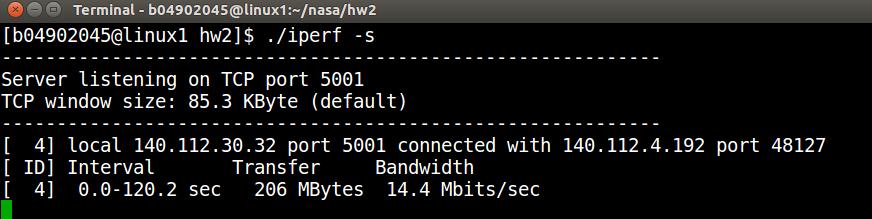
\includegraphics[scale=0.4]{csie_wifi1.png}
                \end{flushleft}
            \end{figure}
        \newpage
        \subsubsection{4G(HTC Portable Hotspot)}
            This is done in CSIE basement, so the 4G signal is pretty weak.
            \begin{figure}[!htb]
                \begin{flushleft}
                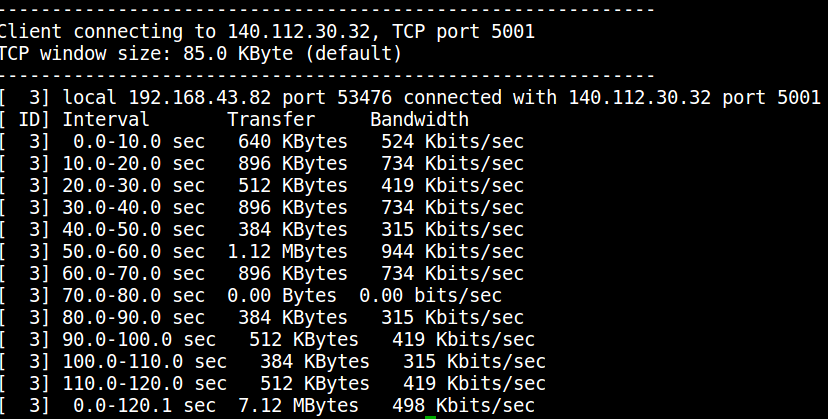
\includegraphics[scale=0.4]{4G.png}
                \end{flushleft}
            \end{figure}
            \begin{figure}[!htb]
                \begin{flushleft}
                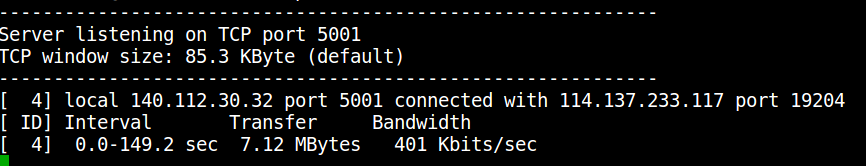
\includegraphics[scale=0.4]{4G1.png}
                \end{flushleft}
            \end{figure}
        \newpage
        \subsubsection{Ethernet with 204 computer}
            \begin{figure}[!htb]
                \begin{flushleft}
                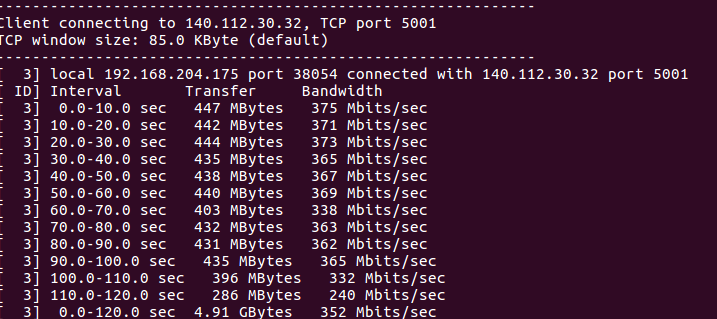
\includegraphics[scale=0.4]{eth0.png}
                \end{flushleft}
            \end{figure}
            \begin{figure}[!htb]
                \begin{flushleft}
                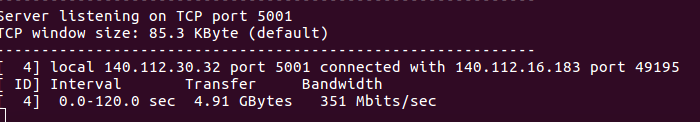
\includegraphics[scale=0.4]{eth1.png}
                \end{flushleft}
            \end{figure}

\end{document}
